% !TEX root = main.tex

\section{Experiments}
\label{sec:experiments}
In this section, we conduct experiments to evaluate the performance of our method on Ethereum transaction graph. Note that AIGL does not only apply to Ethereum, but also other cryptocurrencies based on account/balance model.

\subsection{Data Collection}
We collect all data by running Ethereum client\footnote{Parity Ethereum Client, https://www.parity.io/ethereum/} which maintains the same copy of blockchain with all historical transactions. Note that we choose the transaction logs on Ethereum from January 1, 2018 to March 31, 2018 (116,293,867 external transactions and internal transactions in total) as the input of graph construction since it is the most active period with various activities.

By parsing the transactions, 16,599,825 active accounts are obtained, including 14,450,993 EOAs and 2,148,831 SCs. Then we construct the original ETG based on these accounts and transactions.

Specially, we extend the pre-processing scheme to adapt our model. First we construct four relation graphs, which contains ETH transfer graph, contract creation graph, contract invocation graph and mining reward graph. In each graph, repeated edges between the same node pair are merged via the method introduced in Section \ref{sec:model}.

%Last, a set of accounts with label introduced before is provided to train the model and evaluate classification accuracy. It is hard to reveal the identity of addresses since the anonymity of blockchain. We obtain these labeled examples in two ways, \emph{Etherscan}\footnote{Etherscan LabelCloud, https://etherscan.io/labelcloud} and \emph{Searchain}\footnote{Searchain, http://www.searchain.io/}. In the label set, the number of samples of each category is 100.

\subsection{Identity Categorization}
Since AIGL is semi-supervised learning method, and a small set of labeled accounts should be provided for training. We obtain these labeled examples via \emph{Etherscan}\footnote{Etherscan LabelCloud, https://etherscan.io/labelcloud} and \emph{Searchain}\footnote{Searchain, http://www.searchain.io/}. 

TABLE~\ref{table:identity} shows the taxonomy of Ethereum accounts and here we depict them in detail. Here we introduce the prominent identity tag which is provided to train the model and evaluate classification accuracy.
 %It is hard to reveal the identity of addresses since the anonymity of blockchain.  %In the label set, the number of samples of each category is 100.

\noindent 1) \emph{Miners \& Mining Pools}
The existing implementation of Ethereum blockchain use the \emph{Proof-of-Work (PoW)} protocol, similar with Bitcoin. 
%in which a block is only valid if it contains \emph{Proof-of-Work} (PoW) of a given difficulty\footnote{Note that in the Ethereum Serenity milestone, this is likely going to be replaced by a Proof-of-Stake mechanism.}. 
The \emph{miners} are the individuals or groups who validate transaction information by solving the cryptographic puzzles. Whoever is the first to find a valid hash of block will get the reward in the form of ETH which is paid by users sending transactions. And an efficient solution is working together to solve the PoW problems. Miners with mining machines can register on a special institution named \emph{mining pool}, which aggregates all the registrants' computing power to solve mining problem and distributes the reward to the registrants according to their proportion of contributed computing power. Up to September 2018, top $3$ mining pools occupy more than 65\% of hash rate in Ethereum\footnote{Investoon, https://investoon.com/charts/mining/eth.}.

%In the early stage, most people participate the mining process independently. As more participants into this high profit industry, the mining competition gradually becomes fiercer. 


\noindent 2) \emph{Exchanges}
The exchanges are the platforms for trading ETH and even other digital currencies, which play important roles in Ethereum ecosystem. Most of cryptocurrency trading is done through centralized exchanges such as Binance, Huobi, OKEX, etc\footnote{``Top 100 Cryptocurrency Exchanges by Trade Volume'', https://coinmarketcap.com/rankings/exchanges}. The centralized exchange allocates a deposit address to each user who wants to make transaction in the exchange. These addresses are called \emph{exchange deposits} and belong to the exchange since users do not have the private key of these addresses. In recharge process, user transfers coins to the given deposit address from her own wallet and these coins will be transferred to the \emph{exchange root} address automatically. In turn, users send requests to exchange to withdraw their coins from an address called \emph{exchange withdrawal}. And in most cases, the exchange root and exchange withdrawal mean the same address.

%The exchanges can be categorized into centralized exchanges and decentralized exchanges (also known as DEXs) according to their architectures.

%The exchange charges the user a commission for both recharge and withdraw services.

%The DEXs are a new technology that facilitate cryptocurrency trading on a distributed ledger. Being completely on-chain, all orders interact with each other directly through the blockchain. This makes it fully decentralized, but also expensive and slow. Besides, another difference is that user will get a new address with corresponding private key when registers to the DEX, which means the address belongs to user itself instead of exchange. 
 
 %User calls the smart contract in the decentralized exchange address to start a transaction. Intuitively, the transaction will take a long time for making match and confirming compared with in centralized way.

%Since most ERC-20 token transactions happen via smart contracts and in a decentralized mechanism, some big exchanges which support both ETH and ERC-20 token transaction (e.g., Binance and Huobi) are mixture of centralized and decentralized exchange. 


\noindent 3) \emph{ERC-20 \& ICO}
ERC-20 is a technical standard used for smart contracts on the Ethereum blockchain for implementing tokens~\cite{erc-20-wiki}. It defines a common list of rules that an Ethereum token has to implement, giving developers the ability to program how new tokens will function within the Ethereum ecosystem. Such ERC-20 token transfer happens in specific CA which is called \emph{ERC-20 token contract}. The ERC-20 token standard became popular with crowdfunding companies working on ICO cases due to the simplicity of deployment, together with its potential for interoperability with other Ethereum token standards~\cite{erc-20}. As of July 26 2018, there were more than 103,621 ERC-20 token contracts\footnote{Etherscan Token Tracker Page, https://etherscan.io/tokens}. Among the most successful ERC-20 token sales are EOS, Filecoin, Bancor, Qash, and Nebulas, raising over 60 million each\footnote{``Token Data, data and analytics for all ICO's and tokens", https://www.tokendata.io}.

Participants in the initial ICO round are \emph{investors} who buy the ERC-20 token from ERC-20 smart contracts of the crowdfunding companies. And these addresses where ETH holding of token teams are \emph{ICO wallets}.

\noindent 4) \emph{Phishes \& Hacks}
Since virtual property transactions are now becoming increasingly commonplace and that leads to many security issues. At the same time, the frauds associated with ETH and ERC-20 tokens have also increased. We call these addresses related to frauds \emph{phishes \& hacks}. According to Ethersacan, there are more than $2500$ addresses are labeled as Phish/Hack, which takes up the highest proportion. Most of them are disguised as ERC-20 token sales or DApps such as casino. 

\begin{table}[t]
\caption{Typical Account Identities}
\begin{center}
\begin{tabular}{|p{2.1cm}|c|p{3.9cm}|}
\hline
\textbf{Identity} & \textbf{Account Type}& \textbf{Description} \\
\hline
Miners & EOA & Nodes who take part in the block validation process. \\ \hline
Mining Pools & EOA & The pooling of resources by miners, who share their processing power over a network.\\ \hline
Token Contracts & CA & Contracts that allow customers to transfer ERC-20 tokens. \\ \hline
Investors & EOA & Large holders of ETH, who usually got in early on ICOs. \\ \hline
ICO Wallets & EOA\&CA & ETH holdings of token teams, typically raised from ICOs. \\ \hline
Exchange Deposits & EOA\&CA & Addresses for user to deposit ETH at exchange. \\ \hline
Exchange Roots\&Withdrawals & EOA\&CA & Addresses collect ETH from deposit addresses and withdraw ETH to users. \\ \hline
Phishes\&Hacks & EOA\&CA & Fraud address related to phishing and hacks. \\ \hline
%\multicolumn{4}{l}{$^{\mathrm{a}}$Sample of a Table footnote.}
\end{tabular}
\label{table:identity}
\end{center}
\end{table}

%Phishing is the name given to the latest online scam where millions of unwary Americans are getting their identities stolen.

%We've seen increased use of sophisticated forms and letterhead to send what appears to be legitimate World Bank Group correspondence, as well as several schemes that reference the Bank.



\subsection{Experimental Set-Up}
As a baseline for our experiments, we compare against state-of-the-art classification results from DeepWalk~\cite{perozzi2014deepwalk}, PARW~\cite{wu2012learning} and rGCN~\cite{schlichtkrull2018modeling}. DeepWalk uses random walks on graphs to obtain node representations. Due to DeepWalk is an unsupervised method, a logistic regression model is added for classification. As a label propagation method, PARW is guaranteed to meet the cluster assumption under proper absorption rates. rGCN is a kind of deep neural network based method and can be applied to modeling relational data. 

Unless otherwise noted, all the GCN-based hidden layers have 16 units. Models are trained with Adam optimizer for 100 epochs, and dropout with $dropout\_rate=0.5$ is utilized to avoid overfitting.

\begin{table*}
\footnotesize
\centering
\caption{Identity Classification Results}
\resizebox{\textwidth}{17mm}{
\begin{tabular}{l|ccc|ccc|ccc|ccc|ccc}
\toprule
 & \multicolumn{3}{c|}{DeepWalk} & \multicolumn{3}{c|}{PARW} & \multicolumn{3}{c|}{rGCN} & \multicolumn{3}{c|}{rGCN+asymmetric proximity} & \multicolumn{3}{c}{AIGL} \\
\midrule
& \textbf{Precision} & \textbf{Recall} & $\mathbf{F_1}$ & \textbf{Precision} & \textbf{Recall} & $\mathbf{F_1}$ & \textbf{Precision} & \textbf{Recall} & $\mathbf{F_1}$ & \textbf{Precision} & \textbf{Recall} & $\mathbf{F_1}$ & \textbf{Precision} & \textbf{Recall} & $\mathbf{F_1}$ \\
\midrule
 phish and hack & 0.609 & 0.394 & 0.479 &0.565 & 0.333 & 0.419 & 0.913& 0.212& 0.344& 0.720& 0.727& 0.724& 0.714& 0.758& 0.735\\
 token contract & 0.857& 0.735 & 0.791 &0.354& 0.718& 0.475& 0.908& 0.602& 0.724& 0.958& 0.939& 0.949& 0.958& 0.939& 0.949\\
 exchange deposit & 0.586 & 0.531 & 0.557 &0.692& 0.281& 0.400& 0.688& 0.440& 0.537& 0.615& 0.640& 0.628& 0.556& 0.600& 0.579\\
 exchange root & 0.647 & 0.759 & 0.698 &0.667& 0.759& 0.710& 0.923& 0.686& 0.787& 0.862& 0.714& 0.781& 0.828& 0.686& 0.750\\
 pool & 0.692 & 0.750 & 0.720 &0.789& 0.625& 0.697& 1.000& 0.727& 0.842& 0.842& 0.727& 0.781& 1.000& 0.727& 0.842\\
 miner & 0.400 & 0.694 & 0.508 &0.667& 0.872& 0.756& 0.867& 0.951& 0.907& 0.826& 0.927& 0.874& 0.841& 0.902& 0.871\\
 primary market & 0.405 & 0.548 & 0.466 & 0.727& 0.516& 0.604& 0.739& 0.548& 0.630& 0.680& 0.548& 0.607& 0.750& 0.484& 0.588\\
 ICO wallet & 0.364 & 0.353 & 0.358 & 0.630& 0.500& 0.558& 0.546& 0.158& 0.245& 0.769& 0.526& 0.625& 0.742& 0.605& 0.668\\
 \midrule
 average & 0.614 & 0.583 & \bf{0.585} & 0.623& 0.577& \bf{0.570}& 0.848& 0.496& \bf{0.593}& 0.806& 0.761& \bf{0.779}& 0.811& 0.764& \bf{0.782}\\
\bottomrule
\end{tabular}
}
\label{table:overall_results}
\end{table*}

All embedding and classification programs were run on the server, which includes Intel Xeon E5 CPU with 55 processors and 128GB of memory, and the GPU used for deep learning is Nvidia 1080.

\subsection{Classification Results}
In the first experiment, we test AIGL on classification with the label set. To make the classification more intuitive, there are two assumptions. (1) Account is supposed to have a single identity instead of multiple identities, and (2) identity of a certain account is not easy to change. Reasons for these are that, people who take on many identities, e.g., miner and investor both, tend to hold multiple accounts usually and each account is related to one identity. Besides, as as the time span of data we collected is merely three months, cases of identity conversion is negligible.

We use three indicators to evaluate each model, including precision, recall and $F_1$ score. Precision is the fraction of relevant instances among the retrieved instances, while recall is the fraction of relevant instances that have been retrieved over the total amount of relevant instances. And $F_1$ score is a measure that combines precision and recall, which is computed as
\begin{equation}
F_1=(\frac{{precision}^{-1}+{recall}^{-1}}{2})^{-1}=2\cdot\frac{precision \cdot recall}{precision + recall}
\end{equation}

In statistical analysis of label classification, the $F_1$ score is an important indicator since it is the harmonic average of the precision and recall.

Results are summarized in TABLE~\ref{table:overall_results}. Our methods (with asymmetric proximity only and with asymmetric proximity and time-density both) outperform others in average $F_1$ score. Comparing with DeepWalk and PARW, our methods achieve higher $F_1$ scores in all labels, for these methods only utilize the local structure of nodes, while our methods involve global structural information and statistic information. 

Note that rGCN achieves the highest average precision but a low average recall. Especially, rGCN has the lowest recall of category of phish and hack, which means that many normal accounts are inferred as threatening in rGCN model. Our methods improve the overall performance by adding richer information, the time of transactions, into the model.

%\subsection{Asymmetric Proximity and Time-Density}
\subsection{Visualization and Deeper Analysis}
Because AIGL is a graph deep learning approach based on graph embedding, and each node in the graph can be represented as a low-dimensional vector. It allows us to visualize the nodes and gain a better understanding of classification. Note that PARW is based on label propagation instead of embedding, we illustrate the visualization of DeepWalk, rGCN and our methods in Fig.~\ref{fig:visualization}. Similar to [], we learn a 128-dimensional embedding for each method and input it to t-SNE[] to reduce the dimensionality to 2, then all nodes can be visualized in a 2-dimensional space.

It can be observed that all GCN based approaches outperform DeepWalk since 2-layers GCN models preserve second-order proximity well~\cite{goyal2018graph}. This illustrates the importance of higher order proximity in the structure of transaction graph.

Preserving asymmetric proximity by adjusting the adjacency matrix, our method greatly improves the robustness between different labels. We observe that in vanilla rGCN, performances of different labels vary a lot, but adding asymmetric property solves the problem. % This is because in vanilla rGCN, 

Based on this, the result is better when we take time-density into consideration. Different types of accounts have diverse active time distribution, so time-density helps to distinguish between them. Also, intensive transactions reflect more typical characteristics, therefore deserve higher weights.
 
\begin{figure*}
\centering     %%% not \center
\subfigure[DeepWalk]{\label{fig:a}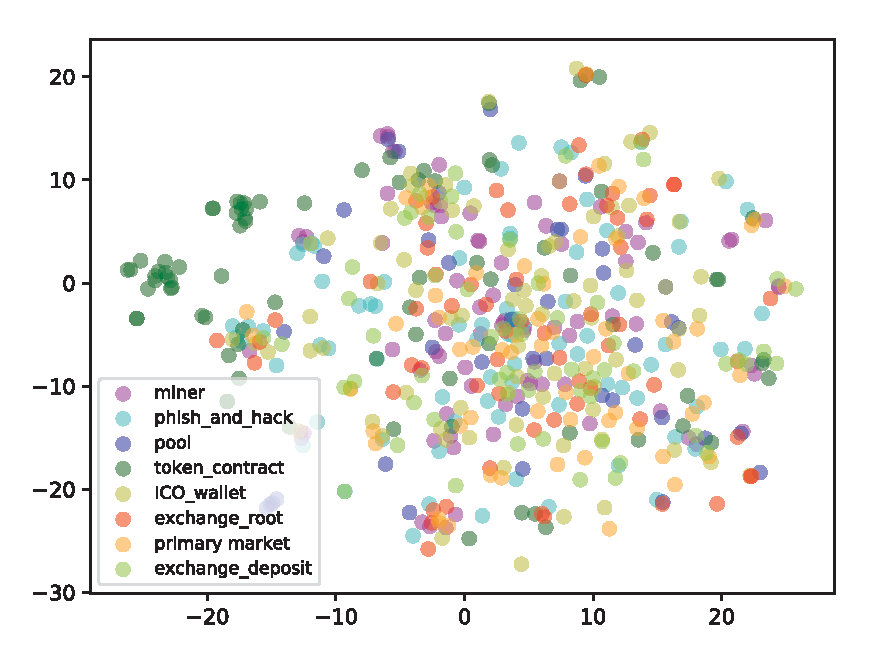
\includegraphics[width=42mm]{fig/rgcn_181_dw_20}}
\subfigure[rGCN]{\label{fig:b}\includegraphics[width=42mm]{fig/rgcn_181_rgcn_20}}
\subfigure[rGCN+asymmetric proximity]{\label{fig:a}\includegraphics[width=42mm]{fig/rgcn_181_rgcn_181_asym_only_20}}
\subfigure[AIGL]{\label{fig:a}\includegraphics[width=42mm]{fig/rgcn_181_rgcn_ours_20}}

\caption{Visualization of nodes with different labels in 2-dimensional space.}
\label{fig:visualization}
\end{figure*}

%%% Local Variables:
%%% mode: latex
%%% TeX-master: "analysis"
%%% End:
